\documentclass[twocolumn]{article}

\usepackage[utf8]{inputenc}
\usepackage{CJKutf8}
\usepackage{CJK}
\usepackage{algorithm}
\usepackage{algorithmic}
\usepackage{amsmath}
\usepackage{amsthm}
\usepackage{amssymb}
\usepackage{newfloat}
\usepackage{setspace}
\usepackage{tikz}
\usepackage{fancyhdr}
\allowdisplaybreaks[4]
\usetikzlibrary{arrows,graphs}
\usetikzlibrary{graphs}
\usetikzlibrary{graphs.standard}
\newenvironment{SChinese}{
	\CJKfamily{gbsn}
	\CJKtilde
	\CJKnospace}{}
\pagestyle{fancy}
\fancyhead[L]{Problem Solving III}
\begin{document}
	\begin{CJK}{UTF8}{}	
		\begin{SChinese}	
			\title{问题求解(三)第10周作业}
			\author{黄奕诚 161220049}
			\maketitle
			
			\section*{TJ Chapter 3}
				\subsection*{3}
					矩形的对称形所构成的群的Cayley表如下:\\
					\begin{tabular}{c|cccccccc}
						$o$ & $id$ & $\rho_1$ & $\rho_2$ & $\rho_3$ & $\mu_1$ & $\mu_2$ & $\mu_3$ & $\mu_4$ \\
						\hline
						$id$ & $id$ & $\rho_1$ & $\rho_2$ & $\rho_3$ & $\mu_1$ & $\mu_2$ & $\mu_3$ & $\mu_4$ \\
						$\rho_1$ & $\rho_1$ & $\rho_2$ & $\rho_3$ & $id$ & $\mu_4$ & $\mu_1$ & $\mu_2$ & $\mu_3$ \\
						$\rho_2$ & $\rho_2$ & $\rho_3$ & $id$ & $\rho_1$ & $\mu_3$ & $\mu_4$ & $\mu_1$ & $\mu_2$ \\
						$\rho_3$ & $\rho_3$ & $id$ & $\rho_1$ & $\rho_2$ & $\mu_2$ & $\mu_3$ & $\mu_4$ & $\mu_1$ \\
						$\mu_1$ & $\mu_1$ & $\mu_2$ & $\mu_3$ & $\mu_4$ & $id$ & $\rho_1$ & $\rho_2$ & $\rho_3$ \\
						$\mu_2$ & $\mu_2$ & $\mu_3$ & $\mu_4$ & $\mu_1$ & $\rho_3$ & $id$ & $\rho_1$ & $\rho_2$ \\
						$\mu_3$ & $\mu_3$ & $\mu_4$ & $\mu_1$ & $\mu_2$ & $\rho_2$ & $\rho_3$ & $id$ & $\rho_1$ \\
						$\mu_2$ & $\mu_4$ & $\mu_1$ & $\mu_2$ & $\mu_3$ & $\rho_1$ & $\rho_2$ & $\rho_3$ & $id$ \\
					\end{tabular}
					共有8个元素。
					\\$(Z_4,+)$群构成的Cayley表如下:\\
					\begin{tabular}{c|cccc}
						$+$ & 0 & 1 & 2 & 3 \\
						\hline
						0 & 0 & 1 & 2 & 3 \\
						1 & 1 & 2 & 3 & 0 \\
						2 & 2 & 3 & 0 & 1 \\
						3 & 3 & 0 & 1 & 2 \\
					\end{tabular}
					\\共有4个元素。\\
					\\由于这两个群含有不同数量的元素,故不同.
					
				\subsection*{6}
					U(12)有4个元素,乘法表格如下:\\
					\begin{tabular}{c|cccc}
						$\cdot$ & 1 & 5 & 7 & 11 \\
						\hline
						1 & 1 & 5 & 7 & 11 \\
						5 & 5 & 1 & 11 & 7 \\
						7 & 7 & 11 & 1 & 5 \\
						11 & 11 & 7 & 5 & 1 \\
					\end{tabular}
				\subsection*{7}
					\begin{proof}
						1.首先证明$(S,*)$是一个群:\\
						(1)首先证明封闭性:因为$S=R\backslash\{-1\}$,对于$a,b\in S$,由于实数本身的封闭性,只要$a\cdot b\neq-1$即可满足封闭性.假设$a\cdot b=-1$,则可以得到$(a+1)(b+1)=0$,即有$a=-1$或$b=-1$,这与$a,b\neq-1$矛盾.因此$a\cdot b\neq-1$,由此满足封闭性;\\
						(2)再证明满足结合律:对任意$a,b,c\in S$,有$(a\cdot b)\cdot c=(a+b+ab)\cdot c=a+b+c+ab+(a+b+ab)c=a+b+c+ab+ac+bc+abc=a\cdot(b+c+bc)=a\cdot(b\cdot c)$,由此满足结合律;\\
						(3)再证明有单位元:假设存在$e\in S$,使得对任意$a\in S$,有$e\cdot a=a\cdot e=e+a+ea$,取$e=0$则成立.因此存在单位元$e$;\\
						(4)最后证明存在逆元:对任意的$a\in S$,若$b\in S$,则$a\cdot b=e$,有$a+b+ab=0$,得$b=-\frac{a}{a+1}$.由于$a\neq-1$,故存在这样的逆元;\\
						综上,$(S,*)$是一个群.\\
						2.又因为对$a,b\in S$,有$a\cdot b=a+b+ab=b+a+ba=b\cdot a$,满足交换律,所以它是阿贝尔群.
					\end{proof}
				\subsection*{17}
					以下三种都互为不同构的8阶群:\\
					(1)$\mathbb{Z}_8$ \\
					(2)$\mathbb{Z}_4\times\mathbb{Z}_2$ \\
					(3)$\mathbb{Z}_2\times\mathbb{Z}_2\times\mathbb{Z}_2$ \\
					\begin{proof}
						第一个群为8阶循环群,每个子群包含一个元素;第二个群的每个子群包含两个元素;第三个群的每个子群包含三个元素.子群结构不同,因此它们互不同构.
					\end{proof}
				\subsection*{28}
					\begin{proof}
						对于(1),$g^mg^n=(\underbrace{g\cdot g\cdot g\cdots g}_{m\textrm{个}})\cdot(\underbrace{g\cdots g\cdot g}_{n\textrm{个}})\\=e(\underbrace{g\cdot g\cdot g\cdots g}_{m\textrm{个}})\cdot(\underbrace{g\cdots g\cdot g}_{n\textrm{个}})\\=e(\underbrace{g\cdot g\cdot g\cdots g}_{m+n\textrm{个}})=\underbrace{g\cdot g\cdot g\cdots g}_{m+n\textrm{个}}=g^{m+n}$\\
						对于(2),$(g^m)^n=\\ \underbrace{(\underbrace{g\cdot g\cdot g\cdots g}_{m\textrm{个}})\cdot(\underbrace{g\cdot g\cdot g\cdots g}_{m\textrm{个}})\cdots(\underbrace{g\cdot g\cdot g\cdots g}_{m\textrm{个}})}_{n\textrm{个}}\\=e\underbrace{(\underbrace{g\cdot g\cdot g\cdots g}_{m\textrm{个}})\cdot(\underbrace{g\cdot g\cdot g\cdots g}_{m\textrm{个}})\cdots(\underbrace{g\cdot g\cdot g\cdots g}_{m\textrm{个}})}_{n\textrm{个}}\\=e(\underbrace{g\cdot g\cdot g\cdots g}_{mn\textrm{个}})\\=\underbrace{g\cdot g\cdot g\cdots g}_{mn\textrm{个}}=g^{mn}$\\
						对于(3),因为$(gh)^n\cdot(h^{-1}g^{-1})^{n}\\=\underbrace{gh\cdot gh\cdot gh\cdots gh}_{n\textrm{个}}\cdot\underbrace{ h^{-1}g^{-1}\cdot h^{-1}g^{-1}\cdots h^{-1}g^{-1}}_{n\textrm{个}}\\=e^n=e$.因此$(gh)^n=(h^{-1}g^{-1})^{-n}$.若$G$是阿贝尔群,则有$gh=hg$,此时$(gh)^n=\underbrace{gh\cdot gh\cdot gh\cdots gh}_{n\textrm{个}}\\=\underbrace{g\cdot g\cdot g\cdots g}_{n\textrm{个}}\cdot\underbrace{h\cdot h\cdot h\cdots h}_{n\textrm{个}}=g^nh^n$.
					\end{proof}
					
				\subsection*{36}
					\begin{proof}
						除零有理数集$Q^*$的单位元为1,因为对于$k\in Z$,有$1\cdot 2^k=2^k$,故1也是$H$的单位元,满足条件1.对于任意的$k_1,k_2\in Z$,有$2^{k_1}\cdot2^{k_2}=2^{k_1+k_2}\in H$,满足条件2.对于任意的$k\in Z$,有$2^{-k}=\frac{1}{2^k}$,即存在逆元,满足条件3.因此$H$是$Q^{*}$的一个子集.
					\end{proof}
				\subsection*{38}
					\begin{proof}
						不妨设$z_1,z_2\in T$,并且$z_1=\cos\theta_1+i\sin\theta_1,z_2=\cos\theta_2+i\sin\theta_2$定义"乘法"运算为$z_1+z_2=\cos(\theta_1+\theta_2)+i\sin(\theta_1+\theta_2)$.并定义"逆元"为$z^{-1}=\cos\theta-i\sin\theta$.\\
						于是,对于任意的$z_1,z_2\in T$,有$z_1\cdot z_2=\cos(\theta_1+\theta_2)+i\sin(\theta_1+\theta_2)$,有$|z_1\cdot z_2|=1$,故$z_1\cdot z_2\in T$.又对于$z^{-1}$,有$|z^{-1}|=\sqrt{\cos^2\theta+\sin^2\theta}=1$,故$z^{-1}\in T$.\\
						因此,$T$是$C^*$的一个子群.
					\end{proof}
				\subsection*{41}
					\begin{proof}
						定义"乘法"运算为矩阵的加法运算,定义矩阵$A$的"逆元"为$-A$.于是,用Proposition 3.10可证:\\
						首先,矩阵\begin{displaymath}
							A=\left [\begin{matrix}
							1 & -1 \\
							0 & -1   
							\end{matrix}\right]
						\end{displaymath}
						有$A\in H$,故$H$非空.对于任意的$h_1,h_2\in H$,有$h_1\cdot h_2^{-1}=h_1-h_2=\left [\begin{matrix}
						a_1-a_2 & b_1-b_2 \\
						c_1-c_2 & d_1-d_2   
						\end{matrix}\right]
						$ 此时$(a_1-a_2)+(d_1-d_2)=(a_1+d_1)-(a_2+d_2)=0$.因此有$h_1h_2^{-1}\in H$.由此可知$H$是$G$的一个子群.
					\end{proof}
				\subsection*{48}
					\begin{proof}
						因为$a,b$是群$G$的两个元素,所以有$ea=a$.因为$a^3=e$,两边同时"乘以"一个$a$,则有$a^4=ea=a$.又因为$a^4b=ba$,所以可得$ab=ba$,得证.
					\end{proof}
				\subsection*{52}
					\begin{proof}
						$(xy)^2=xyxy=xy$\\
						在等式两边左"乘"$y^{-1}x^{-1}$,可得$xy=e$ \\
						在等式两边先左"乘"$x^{-1}$,再右"乘"$y^{-1}$,可得$yx=e$\\
						由此可得$xy=yx$,因此$G$是一个阿贝尔群.
					\end{proof}
			\section*{TJ Chapter 4}
				\subsection*{1}
					\subsubsection*{(a)}
						\textbf{Disprove}
						易知$U(8)=\{1,3,5,7\}$,若以1,3,5,7为生成元,都不能得到$U(8)$,故它不是循环的.
					\subsubsection*{(b)}
						\textbf{Disprove}
						21也是$Z_{60}$的一个生成元,但它不是质数.
					\subsubsection*{(c)}
						\textbf{Disprove}
						假设$g$是有理数群$Q$的一个生成元,则设$g=p/q(q,p\textrm{为非零整数})$,则对于$ng$和$(n+1)g$来说,$Q$中的一个元素,即$\frac{2n+1}{2}g$无法用$g$生成,因此$Q$不是循环群.
					\subsubsection*{(d)}
						\textbf{Disprove}
						暂举不出反例……
					\subsubsection*{(e)}
						\textbf{Prove}
						假设$A$是一个无穷群,则它必有无穷多个子群,因此$A$是有穷群.
				\subsection*{12}
					一个生成元的循环群:$Z_1$,生成元为$1$ \\
					两个生成元的循环群:$Z_6$,加法运算.生成元为$1$和$5$ \\
					四个生成元的循环群:$Z_10$,加法运算.生成元为$1,3,7,9$ \\
					n个生成元的循环群:$Z_m$,其中满足大于等于0,小于$m$,并且与$m$互质的数有$n$个.
				\subsection*{21}
					当$n=5$时,$z=cis(\frac{2k\pi}{5})$.如下图所示:\\
					\begin{figure}[!h]
						\centering
						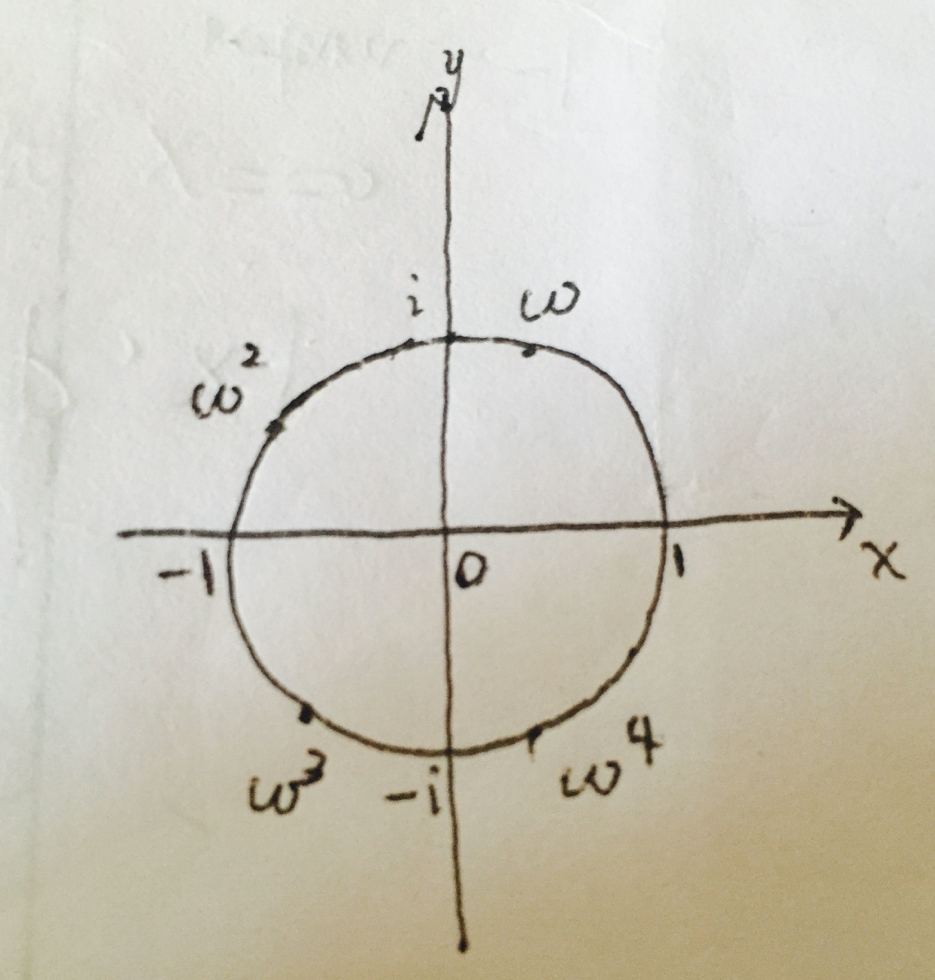
\includegraphics[width=2in,height=2in]{233.png}
					\end{figure}
					设生成元是$\omega$,则列举如下:\\$
						\omega=\frac{\sqrt{5}-1}{4}+\frac{\sqrt{10+2\sqrt{5}}}{4}i\\
						\omega^2=\frac{-1-\sqrt{5}}{4}+\frac{\sqrt{10-2\sqrt{5}}}{4}i\\
						\omega^3=\frac{-1-\sqrt{5}}{4}-\frac{\sqrt{10-2\sqrt{5}}}{4}i\\
						\omega^4=\frac{\sqrt{5}-1}{4}-\frac{\sqrt{10+2\sqrt{5}}}{4}i\\
					$
				\subsection*{24}
					对于任意两个互异的质数$p$和$q$,$Z_{pq}$中的生成元$g$只要满足以下两个条件即可:\\
					(1)$1\le g\le pq-1$\\
					(2)$gcd(g,p)=1$且$gcd(g,q)=1$\\
					考虑到$p,q$为质数,只要不存在正整数$m,n$,使得$g=pn$或者$g=qm$即可.又因为$1\le n\le q-1$且$1\le m\le p-1$,所以只要减去这些情况即可.\\
					因此$Z_{pq}$的生成元个数为$pq-1-(p-1)-(q-1)=pq-p-q+1$.
				\subsection*{32}
					\begin{proof}
						对于$y,y^2,y^3,\cdots,y^n$,只要证明它们互不相同,则可推得其覆盖了$x^0$到$x^{n-1}$的所有值,即生成了$G$.假设存在$y^i=y^j$,则知$x^{ki}=x^{kj}$,即$ki\equiv kj(\mod n)$,也即$k(i-j)\equiv0(\mod n)$.又因为$gcd(k,n)=1$,所以$(i-j)\equiv0(\mod n)$.于是$i=nk+j$,其中$k\in Z$.由此可知在一个周期内,$y,y^2,y^3,\cdots,y^{n-1}$的值互不相等,因此$y$是$G$的一个生成元.
					\end{proof}
			\section*{TJ Chapter 5}
				\subsection*{3}
					\subsubsection*{(a)}
						(14356)=(16)(15)(13)(14)
					\subsubsection*{(b)}
						(156)(234)=(16)(15)(24)(23)
					\subsubsection*{(c)}
						(1426)(142)=(16)(12)(14)
					\subsubsection*{(d)}
						(17254)(1423)(154632)=(14)(15)(12)(17)(13)(16)
					\subsubsection*{(e)}
						(142637)=(17)(13)(16)(12)(14)
				\subsection*{5}
					$S_4$的所有子群为$\{1,2,3,4\}$的所有排列,共有24种.\\
					\subsubsection*{(a)}
						穷举六种情况如下:
						\begin{displaymath}
							\left [\begin{matrix}
							1 & 2 & 3 & 4 \\
							3 & 1 & 2 & 4   
							\end{matrix}\right]
						\end{displaymath}
						\begin{displaymath}
						\left [\begin{matrix}
						1 & 2 & 3 & 4 \\
						3 & 1 & 4 & 2   
						\end{matrix}\right]
						\end{displaymath}
						\begin{displaymath}
						\left [\begin{matrix}
						1 & 2 & 3 & 4 \\
						3 & 2 & 1 & 4   
						\end{matrix}\right]
						\end{displaymath}
						\begin{displaymath}
						\left [\begin{matrix}
						1 & 2 & 3 & 4 \\
						3 & 2 & 4 & 1   
						\end{matrix}\right]
						\end{displaymath}
						\begin{displaymath}
						\left [\begin{matrix}
						1 & 2 & 3 & 4 \\
						3 & 4 & 1 & 2   
						\end{matrix}\right]
						\end{displaymath}
						\begin{displaymath}
						\left [\begin{matrix}
						1 & 2 & 3 & 4 \\
						3 & 4 & 2 & 1   
						\end{matrix}\right]
						\end{displaymath}
						因此,该集合为\\$\{(13),(13)(24),(132),(134),(1324),(1342)\}$
					\subsubsection*{(b)}
						按$(a)$中的穷举法,可以得到集合为$\{(1),(34),(13),(134),(143),(14)\}$
					\subsubsection*{(c)}
						按$(a)$中的穷举法,可以得到集合为$\{(13),(134)\}$
					它们都不是$S_4$的子群.
				\subsection*{16}
					对于正四面体,首先,恒等变换即为$\{(1)\}$;其次,若以顶点与其对立面的面心之连线为轴,每次旋转120度,可以得到3种置换:$\{(12)(34),(13)(24),(14)(23)\}$;以棱心与对棱棱心为轴,进行轴对称置换,可以得到8种:$\{(123),(132),(124),(142),(134),(143),(234),(243)\}$.\\综上所述,正四面体的所有刚体运动群为$\{(1),(12)(34),(13)(24),(14)(23),(123),(132),(124),(142),\\(134),(143),(234),(243)\}$,与$A_4$同构.
				\subsection*{27}
					\begin{proof}
						设$0\le a<n,g\in Z$,欲证$\lambda_g$是$G$的一个排列,即证$\lambda_g$的所有元素都在$G$中,元素个数相同,并且没有重复的元素.对于前两点,由定义$\lambda_g(a)=ga$可直接得出.对于第三点,假设$\lambda_g(a)=\lambda_g(b)$,则有$ga=gb$,即$a=b$,实际上也即$a\equiv b(\mod n)$,说明元素互异.因此,$\lambda_g$是$G$的一个排列.
					\end{proof}
				\subsection*{29}
					$D_8$的中心为本身的单位元$id$以及将正八边形绕中心旋转180度的变换$\{(28)(37)(46)\},\{(13),(48),(57)\},\{(24),(15),(68)\},\\ \{(17),(26),(35)\}$.\\
					$D_10$的中心为单位元$id$以及将正十边形绕中心旋转180度的变换;\\
					$D)_n$的中心,首先都有$id$,若$n$是偶数,则还有将图形绕中心旋转180度的变换;
			\section*{TJ Chapter 6}
				\subsection*{11}
					\subsubsection*{(e)\textrm{推}(d)}
						因为$g_1^{-1}g_2\in H$,所以存在$h\in H$,使得$g_1^{-1}g_2=h$,即$g_2=g_1h$,由此可以推得$g_2\in g_1H$.
					\subsubsection*{(d)\textrm{推}(c)}
						因为$g_2\in g_1H$,所以存在$h\in H$,使得$g_2=g_1h$.设$x\in g_1H$,则存在$h_1\in H$,使得$g_1h_1=x$,也即$x=g_2h^{-1}h_1$,因为$h^{-1}h_1\in H$,故存在$h_2\in H$,使得$x=g_2h_2$,所以$x\in g_2H$,因此$g_1H\subseteq g_2H$.
					\subsubsection*{(c)\textrm{推}(a)}
						再证$g_2H\subseteq g_1H$:设$x\in g_2H$,则存在$h_1\in H$,使得$x=g_2h_1$,于是$x=g_1hh_1$,又$hh_1\in H$,所以$x\in g_1H$,因此$g_2H\subseteq g_1H$,故$g_1H=g_2H$.
					\subsubsection*{(a)\textrm{推}(b)}
						设$x\in Hg_1^{-1}$,则存在$h_1\in H$,使得$x=h_1g_1^{-1}$,因为$g_1h_1=g_2h_1$,故有$g_1=g_2$,代入前式,得到$x=h_1g_1^{-1}=h_1g_2^{-1}$,由此$x\in Hg_2^{-1}$.故$Hg_1^{-1}\subseteq Hg_2^{-1}$,同理可证$Hg_2^{-1}\subseteq Hg_1^{-1}$.因此$Hg_1^{-1}=Hg_2^{-1}$.
					\subsubsection*{(b)\textrm{推}(e)}
						由$Hg_1^{-1}=Hg_2^{-1}$知$Hg_1^{-1}g_2=H$,若$x\in Hg_1^{-1}g_2$,则存在$h_1,h_2\in H$,使得$h_1g_1^{-1}g_2=h_2$,即$g_1^{-1}g_2=h_1^{-1}h_2$.因为$h_1^{-1}h_2\in H$,所以$g_1^{-1}g_2\in H$.
				\subsection*{12}
					\begin{proof}
						设$x\in gH$,则存在$h\in H$,使得$x=gh$,有$x=gh=ghg^{-1}g=hg$.由此$x\in Hg$,所以$gH\subseteq Hg$.同理可知$Hg\subseteq gH$,因此$gH=Hg$. 
					\end{proof}
				\subsection*{16}
					\begin{proof}
						将$G$分为三个部分:$\{e\}$,order为2的元素集$S_1$,order大于2的元素集$S_2$.$x$与其逆元相等当且仅当$x$的order为2或者$x=1$,对于$x\in S_2$,有$x\neq x^{-1}$.又因为$x_1\neq x_2$,即$\textrm{order}(x)=\textrm{order}(x^{-1})$.所以$S_2$的元素个数为偶数.因此,$S_1$的元素个数为偶数-1-偶数,为奇数个.
					\end{proof}
				\subsection*{21}
					\begin{proof}
						设$x$是$G$中非单位元的元素,则由拉格朗日定理知,$x$的阶整除$|G|=p^n$,又因为$p^n$的因数为$p,p^2,\cdots,p^n$,所以$x$的阶只能取其中一个,又因为当$|x|=p^2,p^3,\cdots,p^n$时,可分解为$p$的乘积.因此$G$有一个$p$阶的真子群。当$n\ge3$时,$G$必有一个$p^2$阶真子群.
					\end{proof}
			\section*{TJ Chapter 9}
				\subsection*{6}
					\begin{proof}
						设从$Z_n$到unity第$n$个根的映射为$k\mapsto cis(\frac{2k\pi}{n})$.则有如下一一对应关系:\\
						$1\mapsto cis(\frac{2\pi}{n})$\\
						$2\mapsto cis(\frac{4\pi}{n})$\\
						$\cdots$\\
						$k\mapsto cis(\frac{2k\pi}{n})$\\
						$\cdots$\\
						如此可知它们同构.
					\end{proof}
				\subsection*{7}
					\begin{proof}
						设循环群$G=\{g^n|n\in Z\}$,设从$Z_n$到$G$的映射为$k\mapsto g^k$,则有如下一一对应关系:\\
						$1\mapsto g^1$\\
						$2\mapsto g^2$\\
						$\cdots$\\
						$k\mapsto g^k$\\
						$\cdots$\\
						如此可知它们同构.
					\end{proof}
				\subsection*{8}
					\begin{proof}
						在题目4.1(c)中已证知$Q$对于加法运算不是循环群,而$Z$对于加法运算是循环群,因此它们不同构.
					\end{proof}
				\subsection*{9}
					\begin{proof}
						欲证明$G$是一个定义在$*$运算的群,这个证明过程与题3.7一摸一样,因此不再赘述.下面证明$(G,*)$与非零实数的乘法群同构.\\
						考虑到$a*b=a+b+ab=(a+1)(b+1)-1$,所以$a*b+1=(a+1)(b+1)$,因此对于两个非零实数$a$和$b$,它们的*运算可以与简单乘法一一对应,所以两群同构.
					\end{proof}
			
		\end{SChinese}
	\end{CJK}
\end{document}